\documentclass{article}

\usepackage{authblk}
\usepackage{geometry}
\usepackage{t1enc}
\usepackage[english]{babel}
\usepackage{csquotes}
\usepackage[sorting=none, backend=biber, style=numeric]{biblatex}
\usepackage{graphicx}
\usepackage{caption}
\usepackage{subcaption}

\graphicspath{ {Pictures/} }
\addbibresource{Bibliography/RouteProfileRecording.bib}

\renewcommand\Affilfont{\small}

\geometry{
	a4paper,
	margin=1in}

\title{Methods for recording railway route profiles for vehicle dynamic simulation}

\author{Tamás DEMUS}
\author{Máté M. SZŰCS}
\author{István ZOBORY}
\affil{Department of Railway Vehicles and Vehicle System Analysis\\
Faculty of Transportation Engineering and Vehicle Engineering\\
Budapest University of Technology and Economics\\
H-1111 Budapest, Műegyetem rkp. 3, Hungary}

\date{\today}

\begin{document}
	\pagenumbering{gobble}
	\begin{titlepage}
		\maketitle
		\begin{abstract}
			Railway vehicle dynamics simulation can be performed in several ways. A key factor on the output of such simulation is the parameter set used. Track and vehicle information can be gathered from operators, but control functions are not available in all cases. Identification of these traction and brake control functions is essential. Current research focuses on obtaining those. In this paper a series of measurement is conducted on a selected railway line to record train route profiles which can be used later on to determine the control functions. Focus is put on self-developed tools equipped with GNSS receivers. Field tests carried out and the obtained data is analyzed to compare the different devices used: an iPhone 11 Pro mobile phone and two GNSS receivers applied on the ARDUINO platform. The analysis focuses on the reliability and the achived accuracy of the tools in terms of location, altitude and speed information. A proposal is made which tool to use for extended measurements in the future. The gathered information can be used at a later step of the research to determine track parameters, investigate the realizations and compare with the planned route. \\
			\\
			Keywords: GNSS, railway track, railway vehicle, train positioning, route profile, vehicle dynamics, arduino
		\end{abstract}
	\end{titlepage}	
	\pagenumbering{arabic}
	\section{Introduction}
		Simulating rail vehicle dynamics require reliable input data in terms of track and vehicle parameters and control functions for traction and braking. Obtaining proper control functions difficult as it depends on many factors, such as track condition, vehicle traction mode, driving style, traffic situation or unexpected events. Current research focuses on measurement tools developed to record train route profiles which serves as a basis for determining control functions for later simulations. \\
		The developed tools rely on GNSS technology that is widely used for positioning purposes and subject of extended research in the railway industry. A brief summary about the general application of GNSS technology can be found in \cite{GNSSApplicationsWikipedia}, \cite{GNSSApplicationsNavipedia} while railway applications listed in \cite{RailApplicationsNavipedia} and \cite{salmiInventionsUtilizingSatellite2009}. Current section gives a short overview about the application of GNSS technology for railway track measurements and train positioning and introduces handheld devices developed for solving positioning problems.\\
		Railway track measurement utilizes a range of methods to determine the exact geometry of the track including the position, elevation, curvature, cant, relative position of the rails and so on \cite{MeasuringTestingEquipment}. Common in these methods is that they require measurements done manually and often considered to be a very slow process. To avoid the issue of lengthy measurements GNSS technology is being used to record track geometry. To determine whether the required accuracy can be achieved, extended research program is being carried out at the Gda\'{n}sk University of Technology and the Maritime University of Gdynia as part of the InnoSatTrack project \cite{InnoSatTrackFacultyElectrical}. Several configurations of GNSS receivers studied, results show that accuracy level of 3 mm to 6 mm can be achieved during inventory of railway tracks that allows the study of track deformation \cite{spechtAnalysisTramTracks2017}. It is also indicated that the speed of the receiver during measurement influences the accuracy due to the dynamics of the vehicle, therefore sampling and filtering should be set in a way to allow statistical tools to be used \cite{spechtVerificationGnssMeasurements2020}. For such measurement an increase in accuracy is observed when using multi-mode GNSS receivers \cite{spechtTestingPositioningAccuracy2020}. The research carried out in these projects utilized high-end GNSS receivers with RTK mode and corrections via the GPRS network to mitigate the effect of obstacles around the rail track.\\
		GNSS technology is widely used in not safety critical applications for train positioning. Extended research is in progress to study the application for safety critical applications under the Shift2Rail program \cite{HomeShift2Rail}. An overview of positioning research is given in \cite{oteguiSurveyTrainPositioning2017} and in \cite{spinsanteHybridizedGNSSApproachesTrain2020}. Field research of different technologies and proposal for processing the recorded data is described in \cite{oteguiEvaluationExperimentalGNSS2019}. A specific overview is given in \cite{maraisSurveyGNSSBasedResearch2017} with focus to railway signalling applications. Common in the approach is that GNSS receivers are supported by additional sensors to improve dead reckoning features of the system to avoid signal or accuracy losses. \\
		Several applications of the GNSS technology can be found using low-cost GNSS receivers in combination of small electronic control units, for example the ARDUINO platform \cite{ArduinoHome}. These low-cost solutions can be used for simple tasks, for example positioning and tracking of cars or anti-theft solutions. Some examples can be found in these articles: \cite{costanzoArduinoBasedSystem2013}, \cite{mokhinRealTimeVehicleTracking2018}, \cite{molooLowCostMobileGPS2011}, \cite{moralloVehicleTrackerSystem2021} or \cite{rahmanRealTimeGoogle2016}. Common in these solutions that they utilize a GSM module to transfer the data via the mobile network to the user. Besides these small electronics the opportunity of using the GNSS receivers built-in to mobile phones is also targeted by research work. A comparison of different mobile phones in terms of accuracy can be found in \cite{szotComparativeAnalysisPositioning2019}.\\
		Target of the current study is to develop low-cost solution for recording route profiles of trains. The recorded data later will be used in several different ways:
		\begin{itemize}
			\item Calculate the track parameters of elevation, curvature
			\item Determine maximum allowed speed
			\item Estimate traction and brake force and their control functions
			\item Compare recorded realizations of route profiles with results of numeric simulation and planned profile
			\item Extend measurement scope to different routes to investigate the effect of different parameters of the railway transportation, track and vehicle system
		\end{itemize}
		To achieve these goals the results of the current study has to be evaluated further during later steps in the research. As a first step the following assumptions and considerations have been taken:
		\begin{itemize}
			\item Low-cost and easily available components to be used
			\item No interruption to the railway traffic is possible to obtain real realizations
			\item No GSM connection considered, data is stored in an SD card, therefore augmentation via Internet or GSM network is not possible
			\item No additional sensors are installed to limit complexity and cost level of the system, therefore dead-reckoning is very limited
			\item Different sampling frequencies to be used to evaluate the influence
			\item Processing of data is done off-line
			\item Different protocols can be used for different receivers
		\end{itemize}
	\section{Methodology}
		\subsection{Track and vehicle}
			The line no. 80 and 80a between Budapest-Keleti and Füzesabony stations was selected for the trial measurements (Figure \ref{fig:line_no80}). The line is operated by MÁV-START Co. and part of the Budapest-Keleti to Eger route. It has two standard gauge track with an electrification of 25kV and 50 Hz. The Inter Regio type of train was selected for the measurements which has 10 stops during this section and consits of 2 STADLER FLIRT EMUs coupled together except for the early and late times of the day with an overall of 16 pairs of trains every day. The ride takes 1 hour and 31 minutes, the route is 125 km long and can be divided into three main sections:
			\begin{enumerate}
				\item Budapest-Keleti to Rákoscsaba: lower speed limits, urban area of Budapest, many obstacles around the railway tracks
				\item Rákoscsaba to Hatvan: Gödöllő Hills area, curves with lower radius, wooded area
				\item Hatvan to Füzesabony: plain area, no obstacles, mainly straight sections
			\end{enumerate}
			The section between Rákos and Hatvan is recently renovated and thus giving good track condition. The EMUs are relatively new ones resulting in a good running characteristics offering a good comparison opportunity between the first two sections and the third one.
			\begin{figure}[h]
				\centering
				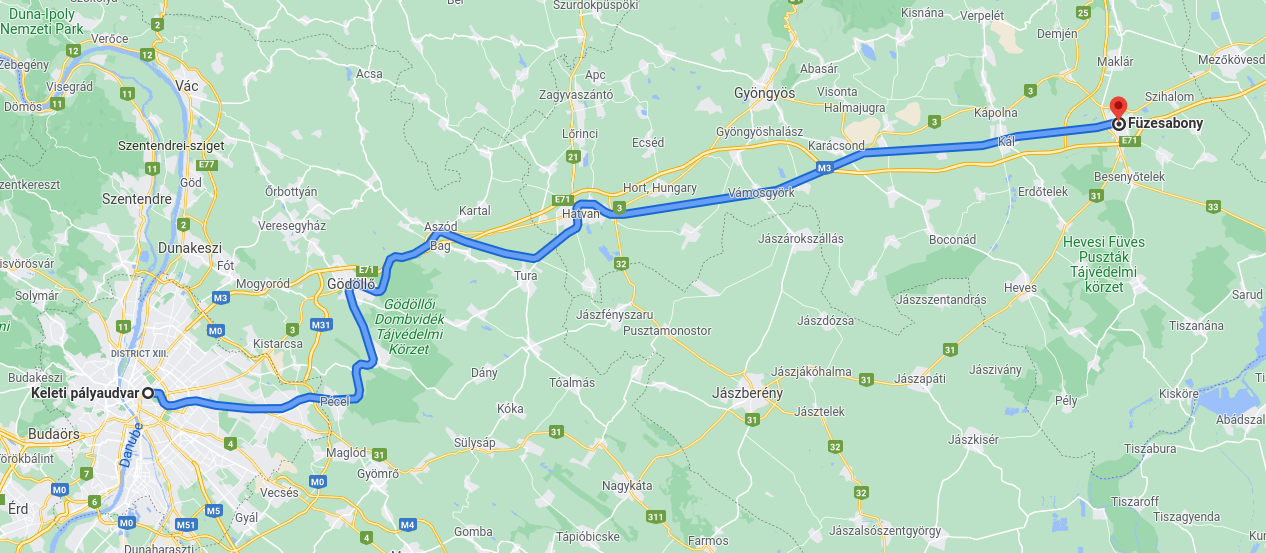
\includegraphics[width=0.9\textwidth]{line_no80.png}
				\caption{Line no. 80 - Budapest-Keleti to Füzesabony}
				\label{fig:line_no80}
			\end{figure}
		\subsection{Measurement devices}
			Three devices were used to carry out the measurements: a mobile phone and two self-made electronics based on the ARDUINO platform but with different GNSS receivers. \\
			The mobile phone type is iPhone 11 Pro with iOS 14 operating system. The application Trail Tracker 1.3.4 was used for the measurements. There is no detailed information available on the type of GNSS receiver used, however from the recorded data we can deduct that the sampling frequency is 1 Hz when a satellite fix is found and multi-mode operation is enabled. The app records and stores the data in GPX format \cite{GPXSchemaDocumentation} that is later used for processing off-line. \\
			The first self-made equipment (Gadget 1) is built from an ARDUINO UNO motherboard and the NEO-M8N receiver made by U-Blox \cite{NEOM8SeriesUblox} and is shown on Figure \ref{fig:gadget1}. An active GNSS antenna is connected to the receiver. The data is recorded to an SD card. The power supply for Gadget 1 is a high-capacity power bank to allow numerous and long test runs. The algorithm for the tool is developed in the ARDUINO IDE environment. It starts by initializing the communication on the serial port, with the receiver and with the SD card. The setup of the GNSS receiver is set to 5 Hz sampling rate and the NMEA messages are disabled. The UBX protocol \cite{UbloxUbloxM82021} is used for the communication between the receiver and motherboard. The UBX-NAV-PVT message is used for transmitting the GNSS information from the receiver that is sent out with a 5 Hz rate. This solution provides general navigation, position, velocity and time information. The messages then parsed by the software and the recorded information is written to the SD card line by line. \\
			The second tool (Gadget 2) is also based on an ARDUINO UNO motherboard but with a combination of an MT 3339 GNSS receiver made by MediaTek Labs \cite{MT3339MediaTekLabs}. The receiver has an active antenna attached. The power supply is solved by the same high-capacity power bank and the data is also recorded to an SD card. In this case the GNSS receiver and the SD card was available in an integrated shield design \cite{OverviewAdafruitUltimate} resulting in a simpler design of the electronics. Gadget 2 is presented on Figure \ref{fig:gadget2}. The software is written in the ARDUINO IDE environment, for the communication the NMEA messages, more precisely the \$GPGGA and \$GPRMC sentences were used which were parsed with 10 Hz sampling rate by the TinyGPSPlus parser \cite{TinyGPSArduiniana} that is freely available. The parsed data was saved to the SD card line-by-line. \\
			For convenient measurements Gadget 1 and Gadget 2 is placed to an aluminium briefcase. The recordings with all tools were done parallel therefore a comparison of the recorded data is possible. Table \ref{table:toolparams} summarizes the main parameters of the tools, the recorded dataset for each solution can be found in Table \ref{table:datasets}. The dataset is different for each tool due to the different software solution applied, this can be unified at a later step of the research.
			\begin{figure}[h]
		   		\centering
		     	\begin{subfigure}[b]{0.45\textwidth}
		      		\centering
		      	  	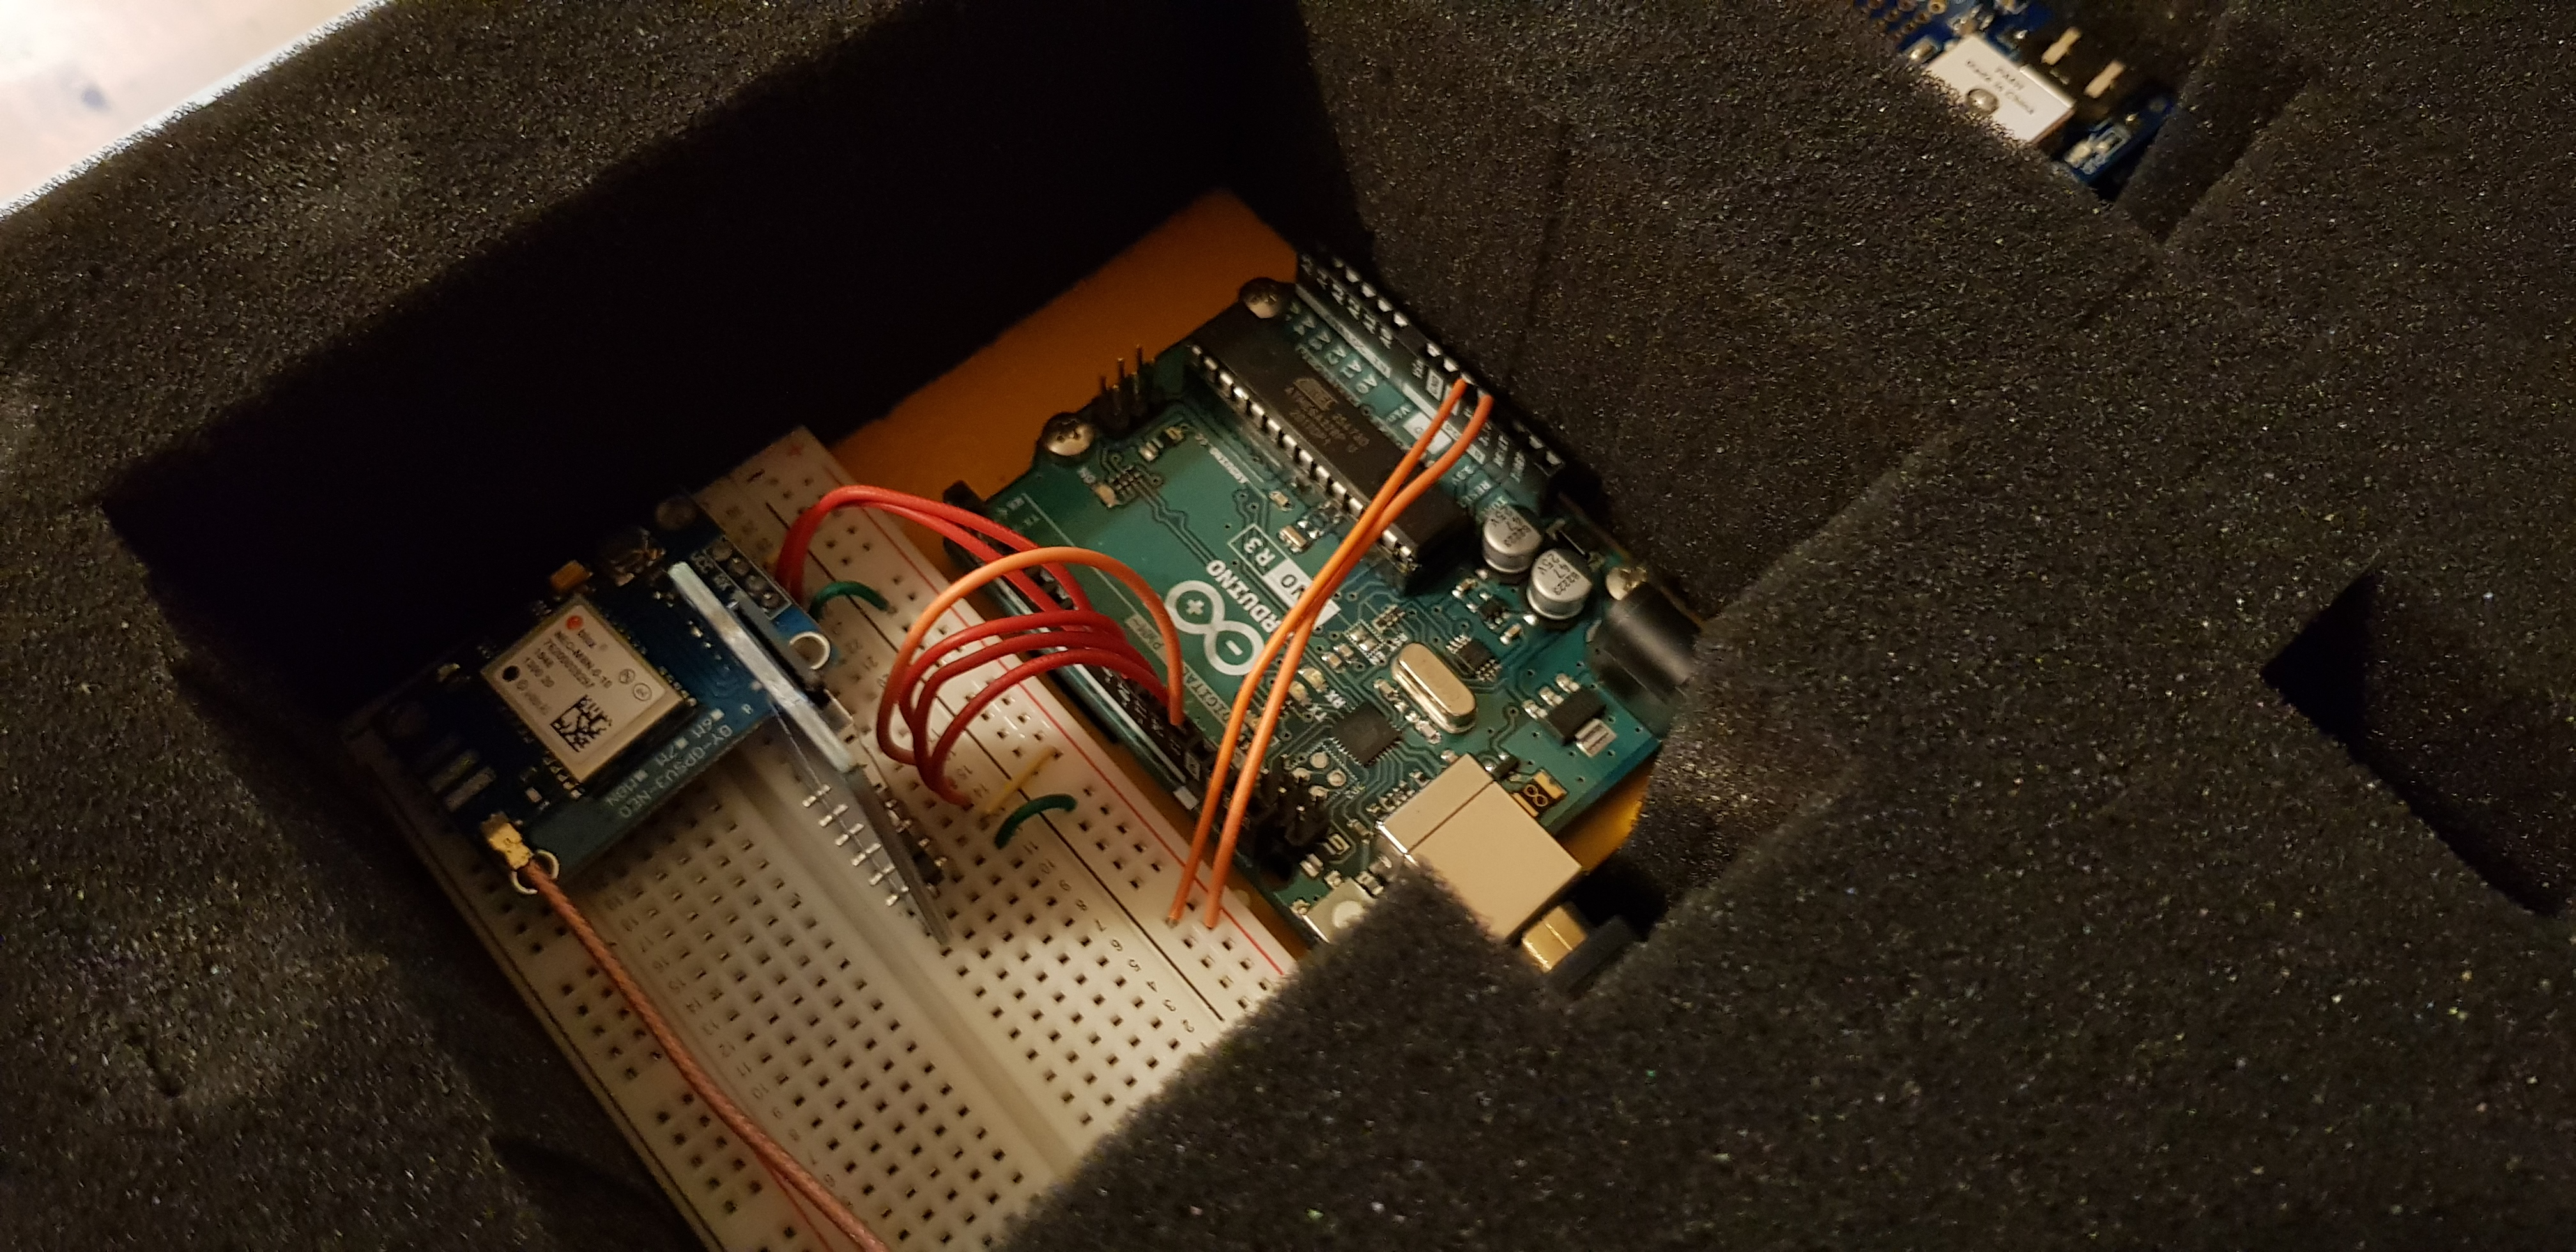
\includegraphics[width=\textwidth]{gadget_1.jpg}
		      	   \caption{Gadget 1}
		      	   \label{fig:gadget1}
		     	\end{subfigure}
		     	\begin{subfigure}[b]{0.45\textwidth}
		      	   \centering
		      	   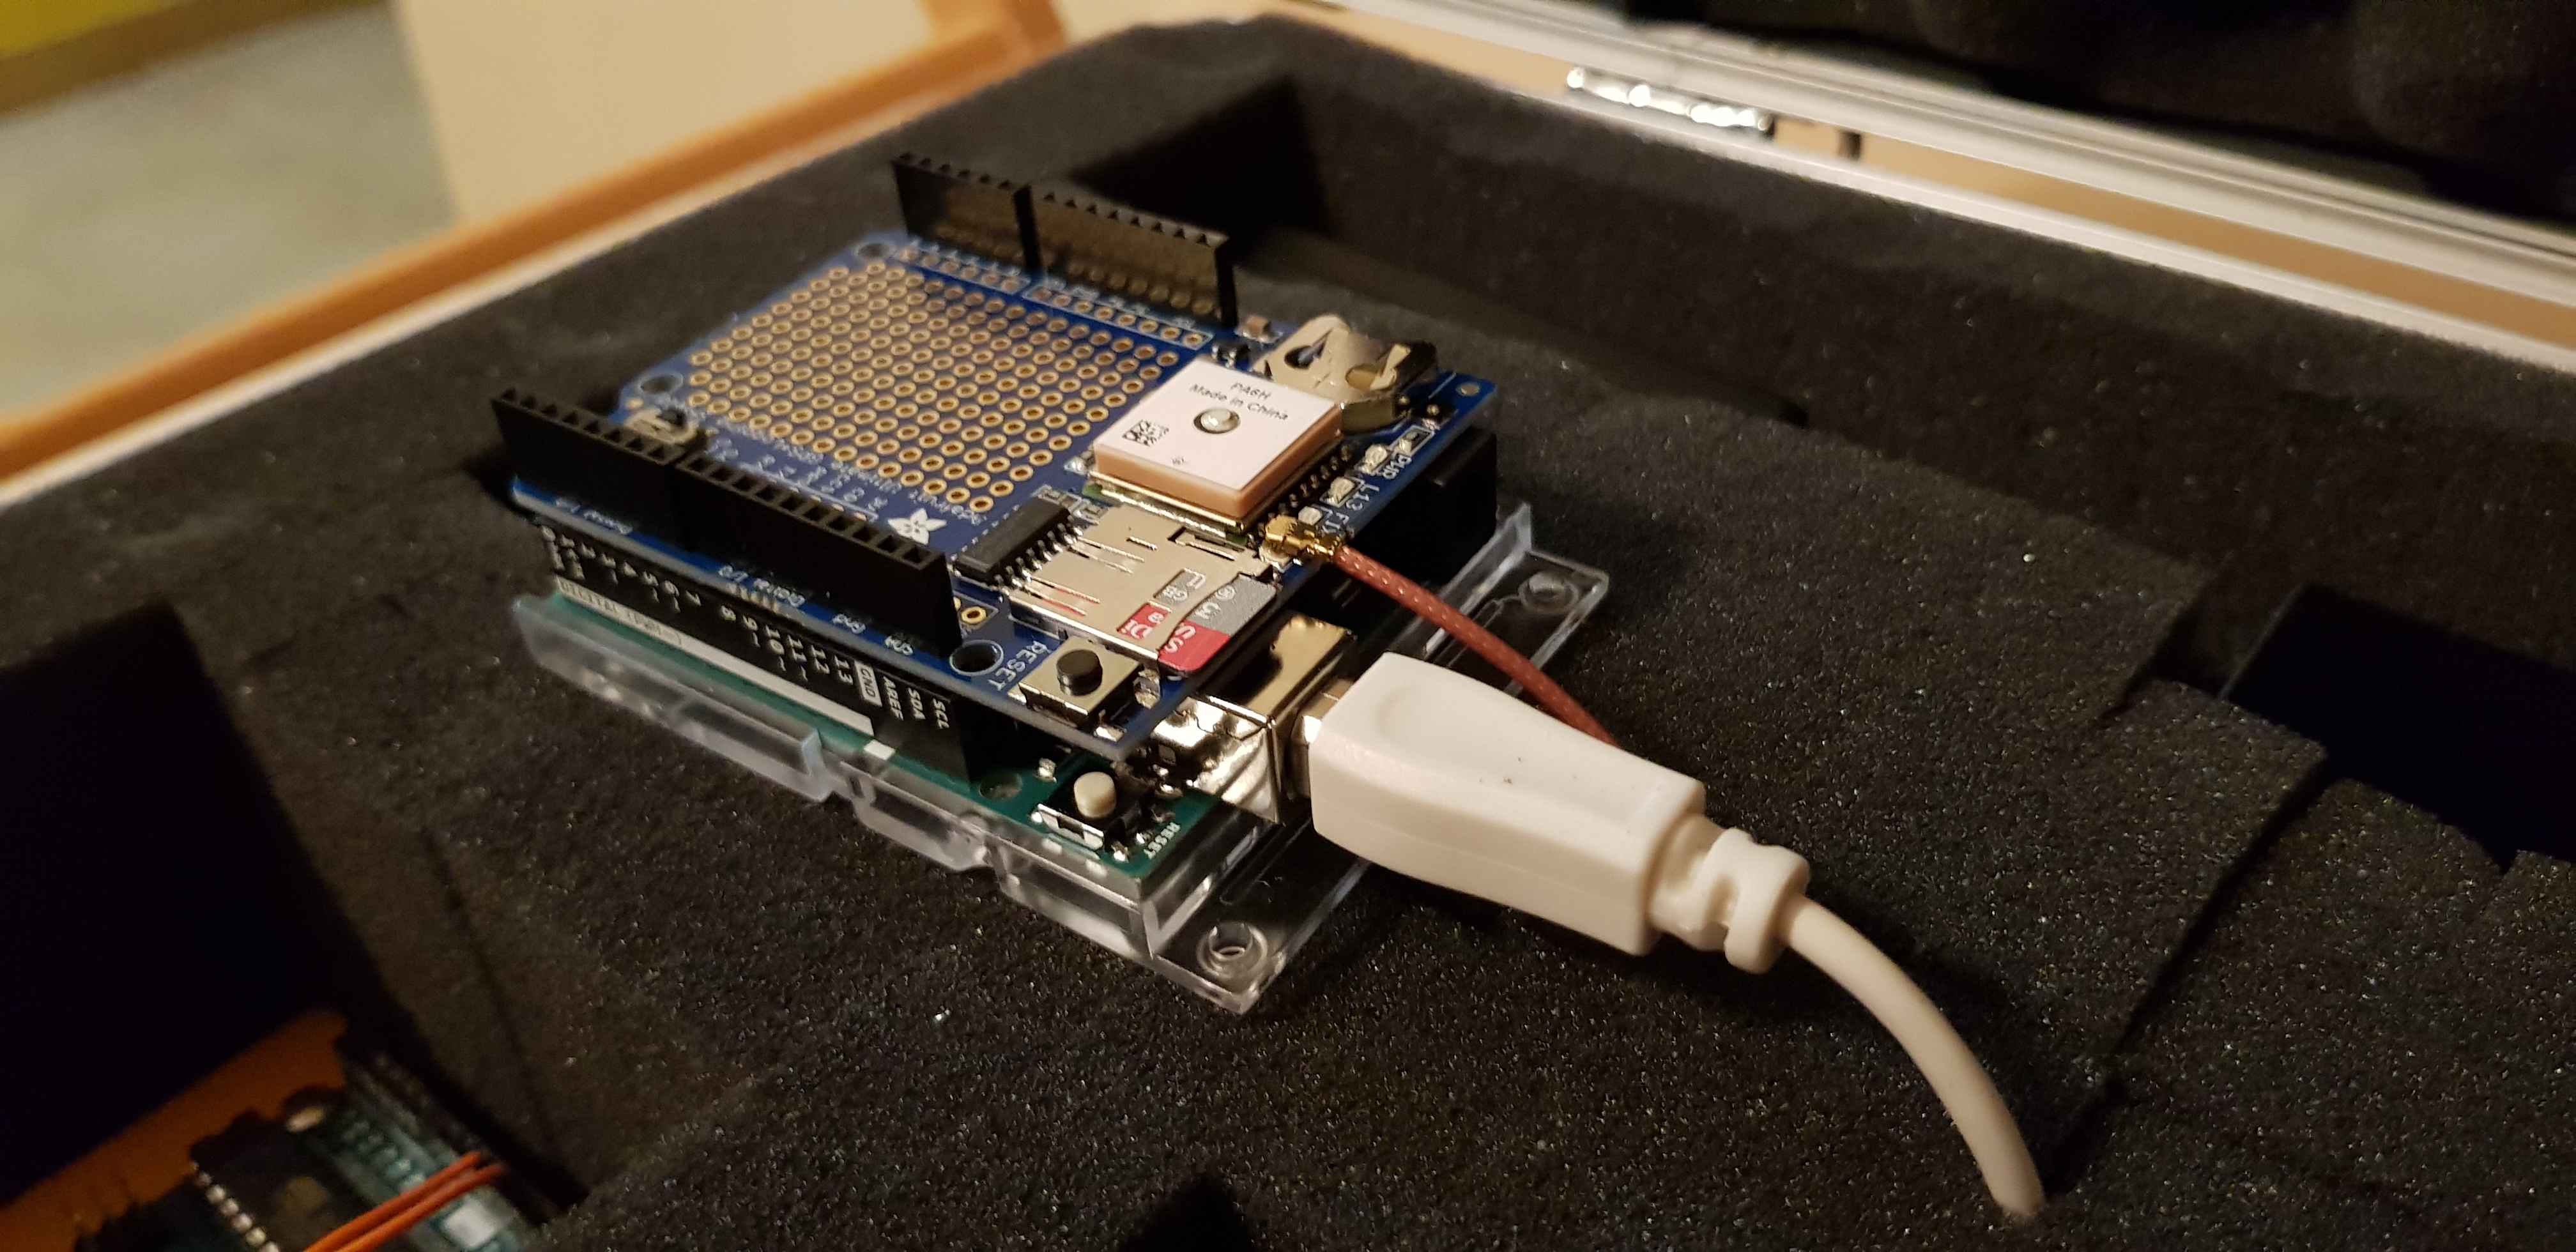
\includegraphics[width=\textwidth]{gadget_2.jpg}
		      	   \caption{Gadget 2}
		      	   \label{fig:gadget2}
		     	\end{subfigure}
		      \caption{Gadget 2}
		      \label{fig:gadgets}
			\end{figure}		
			\begin{table}[h]
				\centering
				\begin{tabular}{|c|c|c|c|}
					\hline 
					& Mobile phone & Gadget 1 & Gadget 2 \\ 
					\hline 
					Hardware & iPhone 11 Pro & ARDUINO UNO & ARDUINO UNO \\ 
					\hline 
					GNSS receiver type & Built-in & U-Blox NEO-M6N & MediaTek Labs MT 3339 \\ 
					\hline 
					Antenna & internal & active external & active external \\ 
					\hline 
					Operating system & iOS 14 & self-made & self-made \\ 
					\hline 
					Recording software & Trail Tracker 1.3.4 & self-made & self-made \\ 
					\hline 
					Communication messages & not known & UBX-NAV-PVT & \$GPGGA \$GPRMC \\ 
					\hline 
					Parser & built-in & self-made & TinyGPSPlus \\
					\hline 
					Sampling rate & 1 Hz & 5 Hz & 10 Hz \\ 
					\hline 
					File format & GPX & CSV & CSV \\ 
					\hline 
				\end{tabular} 
				\caption{Overview of tool parameters}
				\label{table:toolparams}
			\end{table}
			\begin{table}[h]
				\centering
				\begin{tabular}{|c|c|c|c|}
					\hline 
					& Mobile phone & Gadget 1 & Gadget 2 \\ 
					\hline 
					Longitude & X & X & X \\ 
					\hline 
					Latitude & X & X & X \\ 
					\hline 
					Altitude & X & X & X \\ 
					\hline 
					Date & X & X & X \\ 
					\hline 
					Time & X & X & X \\ 
					\hline 
					Speed & X & X & X \\ 
					\hline 
					Number of satellites & & X & X \\ 
					\hline 
					Horizontal dilution of precision & X & & X \\ 
					\hline 
					Vertical dilution of precision & X & & \\
					\hline 
					Position dilution of precision & & X &  \\ 
					\hline 
				\end{tabular} 
				\caption{Recorded data sets}
				\label{table:datasets}
			\end{table}
		\subsection{Data processing}
			The recorded data is processed further with a script developed in Python programming language. During the post-processing of the data three different status of the processing is distinguished. Raw data refers to the recorded data without any alteration. Conditined data refers to the status after general data cleansing is done. Aggregated data refers to the status where the information of the single recorded journeys merged together for each tool separately. \\
			The data cleaning process aims to find single data points that needs to be excluded from further processing, for example speed information recorded above the maximum allowed speed of the vehicle or corrupted data points. The first step is to identify and drop if any corrupted data is present in the time series of the recordings. 
			Second step of the conditioning is to remove highly uncertain points from the evaluation therefore the dilution of precision (DOP) information is analyzed and measurement points with DOP value above 20 are removed as these considered to be inaccurate according to \cite{tahsinAnalysisDOPIts2015}. Low number of satellites present for a GNSS fix is removed due to low accuracy. The minimum number of satellites of 7 is selected for the current study. 
			The remaining time series then analyzed for outliers by calculating the rolling means. The rolling means are used to normalize the recorded values and the standard deviation of the normalized series calculated. The treshold is that each recorded point has to be in \textpm 3 standard deviation range. The calculation is performed for the longitude, latitude, altitude and speed values. Once all the corrupted and outlying points are removed a Savitzky-Golay filter was applied to the series to smooth the dataset as proposed by \cite{wilkDigitalFilteringRailway2020}. At this point the conditioned dataset is produced. \\
			Increasing the number of points for a later statistical analysis on the stochastic behaviour of the route realizations requires several recordings to be done under similar conditions as far as possible. The resulting realizations needs to be aligned to each other. As no reference point of the measurements given the offset between the different realizations need to be determined. This can achieved by searching the maximum value of the correlation for the position locations of the realizations. This can be done in all three dimensions for longitude, latitude and altitude as a function of the distance travelled and then an average value can be taken. The resulting offset applied to the distance values will lead to the aligned set of realizations. Merging all these realizations into a single series results in position coordinates accompanied with speed and altitude information. This is referred as aggregated dataset and allows statistical analysis of the longitude, latitude, altitude and speed values.		
		\subsection{Assessment method}
			A static measurement is carried out to assess the accuracy of the positioning of each tool as described in \cite{szotComparativeAnalysisPositioning2019}. The equipment is placed outside in an area free from obstacles and position information is recorded. The test duration is defined as 12 hours and the accuracy is defined as R68 and R95 for both 2D and 3D. R68 and R95 refers to the radius of the circle (2D) or sphere (3D) that includes the 68\% and 95\% of measurement points respectively. 
			A dynamic measurement is also done, data is recorded while driving a car with stable speeds. Different speeds are selected and the recorded speed profile is compared. This allows the estimation of the accuracy of speed measurement in stable conditions. 
			Train ride recordings taken to assess how the tools work under railway conditions. A single ride is selected and analyzed in terms position, altitude and speed profile for each tool. An aggregated dataset is prepared to analyze the impact of increasing the number of route profiles recorded. Resulting averaged values for position, altitude and speed is compared between the tools. 
			An overview on the number of satellites used for the data recording and the resulting DOP values presented for assessing the achieved accuracy and to allow comparison with different GNSS positioning results.
	\section{Results}
		\subsection{Static test}
		\subsection{Dynamic test}
		\subsection{Position measurements}
			A single route profile for the assessment is selected starting at Füzesabony station, heading to Budapest-Keleti station. The route section in this case starts at the plain section then approaching the hilly area of Gödöllő and arriving to the urban area of Budapest. The location raw and conditioned data is presented on Figure \ref{fig:raw_map} and Figure \ref{fig:cond_map} respectively. It can be seen that the raw data provided a good tracking of the position over the full route profile. The iPhone location data were not so accurate as the recordings with Gadget 1, especially on the second section at Gödöllő Hills. After data cleansing and filtering as the less accurate points were removed the location of the iPhone show larger deviation compared to the recordings of Gadget 1. Both for the iPhone and Gadget 1 the first and third section, the urban area and the plain area respectively resulted in a comparable tracking of the location with limited differences of the location information. The receivers found the satellite signals in a couple of minutes and there was no loss of signal experienced.
			\begin{figure}[h]
				\centering
		      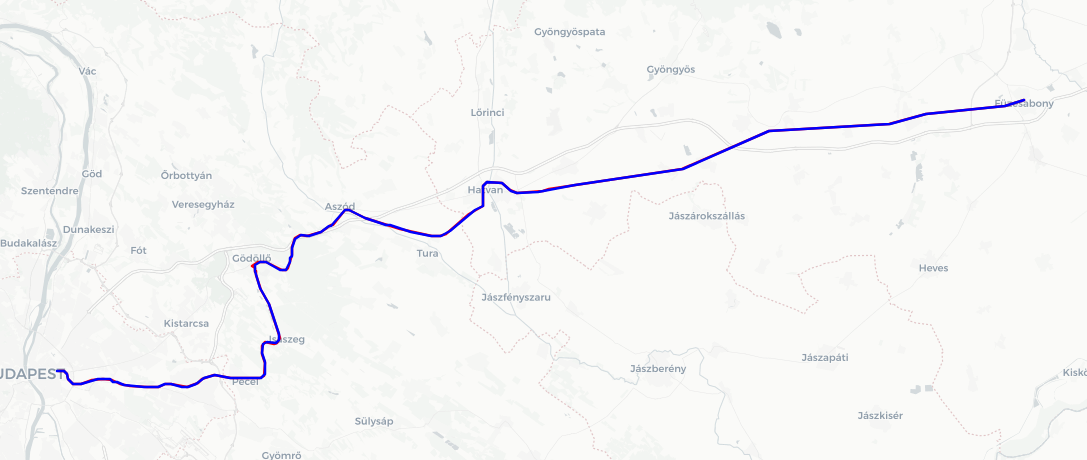
\includegraphics[width=0.9\textwidth]{raw_map.png}
		      \caption{Position from raw data}
		      \begin{tabular}{c c c}
			   		\footnotesize (Red - iPhone 11 Pro & \footnotesize Blue - Gadget 1 & \footnotesize Green - Gadget 2)
		      \end{tabular} 
		      \label{fig:raw_map}
			\end{figure}
			\begin{figure}[h]
				\centering
		   		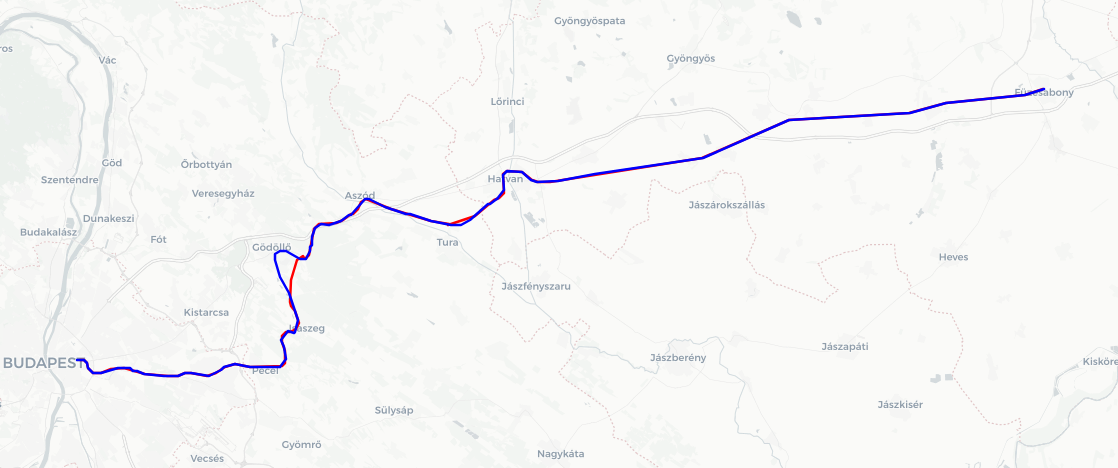
\includegraphics[width=0.9\textwidth]{cond_map.png}
		   		\caption{Position from conditioned data}
		   		\begin{tabular}{c c c}
					\footnotesize (Red - iPhone 11 Pro & \footnotesize Blue - Gadget 1 & \footnotesize Green - Gadget 2)
		      \end{tabular} 
		      \label{fig:cond_map}
			\end{figure}
		\subsection{Altitude measurements}
			Altitude data before and after the data conditioning algorithm is shown in Figure \ref{fig:raw_alt} and Figure \ref{fig:cond_alt}. Clear difference between the recordings of iPhone and Gadget 1 can be observed. The iPhone supplied data with much less variation while the recordings of the Gadget 1 varies in a much bigger interval greatly exceeding the usual gradients of the railway track. Removing the outliers and filtering the dataset the graph become more smooth, the variation of the Gadget 1 data is reduced. Similar effect was observed for the iPhone recording. Additionally the top of the Gödllő Hills, the peak of the altitude is removed from the iPhone dataset. Variation of the Gadget 1 dataset has the same trend that was recorded with the iPhone.
			\begin{figure}[h]
				\centering
			   	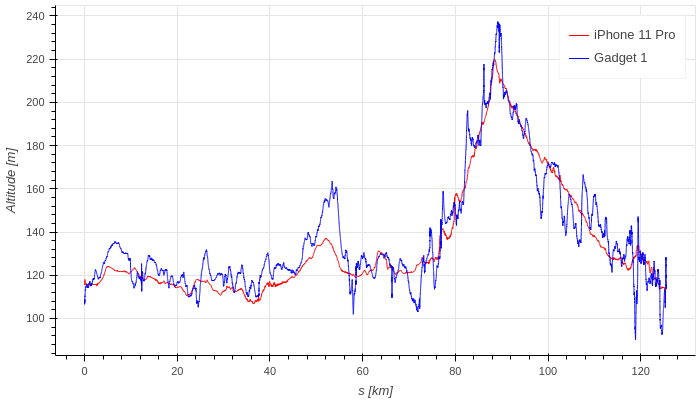
\includegraphics[width=0.9\textwidth]{raw_alt.png}
			   \caption{Altitude from raw data}
			   \label{fig:raw_alt}
			\end{figure}
			\begin{figure}[h]
				\centering
			   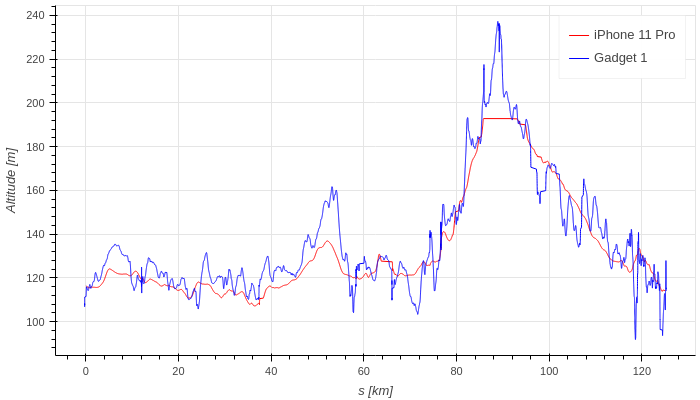
\includegraphics[width=0.9\textwidth]{cond_alt.png}
			   \caption{Altitude from conditioned data}
			   \label{fig:cond_alt}
			\end{figure}
		\subsection{Speed measurements}
			The registered speed values for the raw and conditioned data is shown on Figure \ref{fig:raw_speed} and Figure \ref{fig:cond_speed} respectively. On the raw data several outliers can be identified that are exceeding the vehicle maximum speed (160 km/h) and the allowed maximum speed of the tracks (120 km/h). The outliers belong to the data recorded by the iPhone, while the Gadget 1 contains no outliers. After removing these data and applying the Savitzky-Golay filter, the speed profile is obtained. Well corresponding signals can be seen however some observations can be done. All ten stations can be identified for Gadget 1 while iPhone 11 misses some of them. At some points, where the outliers have been removed the speed profile is also lost. This concentrates on the Gödöllő Hills, part of the second section of the route. Some phase shifting can be seen between the two tools towards the end of the recorded profile that corresponds to the urban area of Budapest. On the plain area (which is in this case the beginning of the route) good correlation can be observed between the profiles.
			\begin{figure}[h]
				\centering
		      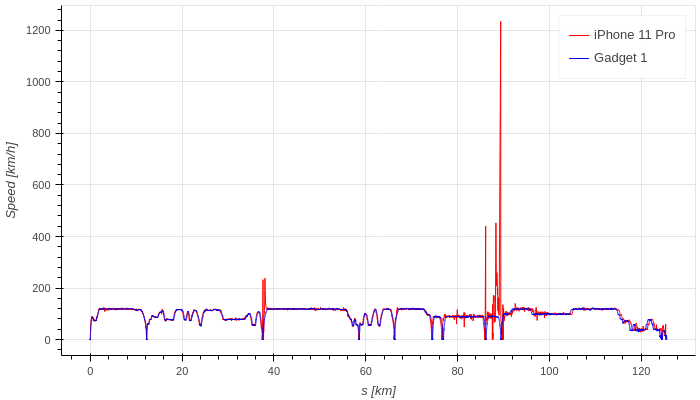
\includegraphics[width=0.9\textwidth]{raw_speed.png}
		      \caption{Speed from raw data}
		      \label{fig:raw_speed}
			\end{figure}
			\begin{figure}[h]
			   \centering
		      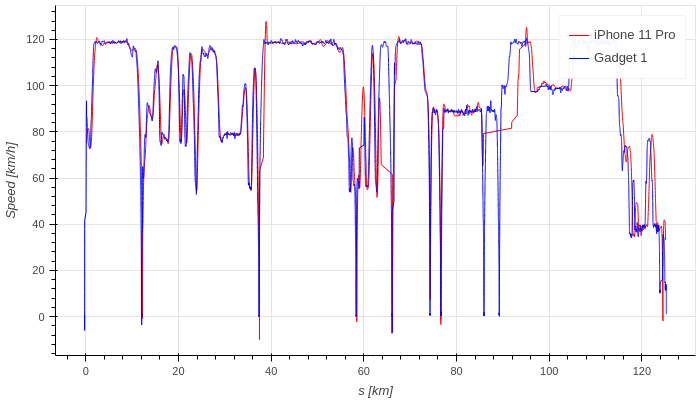
\includegraphics[width=0.9\textwidth]{cond_speed.png}
		      \caption{Speed from conditioned data}
		      \label{fig:cond_speed}
			\end{figure}
		\subsection{Dilution of precision and number of satellites}
			In order to describe the accuracy of the measurements the dilution of precision (DOP) values and the number of satellites are presented in Figure \ref{fig:iPhone_dop} and Figure \ref{fig:Gadget1_dop}. In case of the iPhone the horizontal and vertical DOP values are available. Stable low values can be found in the beginning of the route which increases greatly at the middle section of Gödöllő Hills and then reduces at arriving to Budapest. After clearing the data we can deduct that the horizontal DOP values range between 5 and 20 and the vertical DOP values range between 1 and 5. The results of the Gadget 1 measurement shows the number of satellites, mostly over 9 satellites considered for positioning, also the positional DOP is highlighted which shows low rates but a steady increase on the way to Budapest. After removing the outlyers the number of satellites range between 6 and 14 and the positional DOP changes between 1 and 5, mostly fluctuating around 2.
			\begin{figure}[h]
		   		\centering
		     	\begin{subfigure}[b]{0.45\textwidth}
		      		\centering
		      	   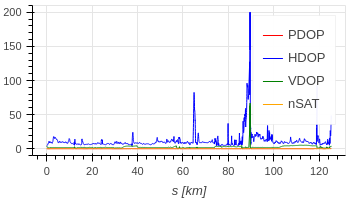
\includegraphics[width=\textwidth]{raw_dop_0.png}
		      	   \caption{Raw data}
		      	   \label{fig:iPhone_raw_dop}
		     	\end{subfigure}
		     	\begin{subfigure}[b]{0.45\textwidth}
		      	   \centering
		      	   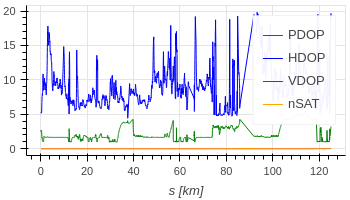
\includegraphics[width=\textwidth]{cond_dop_0.png}
		      	   \caption{Conditioned data}
		      	   \label{fig:iPhone_cond_dop}
		     	\end{subfigure}
		      \caption{iPhone 11 Pro - DOP and number of satellites}
		      \label{fig:iPhone_dop}
			\end{figure}
			\begin{figure}[h]
		    	\centering
		     	\begin{subfigure}[b]{0.45\textwidth}
		      		\centering
		      	   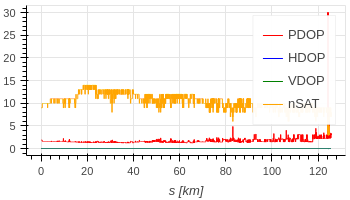
\includegraphics[width=\textwidth]{raw_dop_1.png}
		      	   \caption{Raw data}
		      	   \label{fig:Gadget1_raw_dop}
		     	\end{subfigure}
		     	\begin{subfigure}[b]{0.45\textwidth}
		      	   \centering
		      	   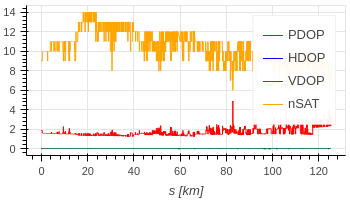
\includegraphics[width=\textwidth]{cond_dop_1.png}
		      	   \caption{Conditioned data}
		      	   \label{fig:Gadget1_cond_dop}
		     	\end{subfigure}
		      \caption{Gadget 1 - DOP and number of satellites}
		      \label{fig:Gadget1_dop}
			\end{figure}
		\subsection{Aggregated figures}
	\section{Discussion}
		The comparison of the recorded datasets shows in general that the Gadget 1 is providing more accurate positioning and speed information than the iPhone 11 Pro. This is confirmed by the geographical location as no differences can be seen on the Gadget 1 compared to the railway tracks than the location provided by the iPhone. Although the deviation to the exact railway track trajectory is not quantified as no information is available that would allow this, the comparison with Google Maps and the continuity of the trajectory supports this observation. \\
		On the other hand contradictory results obtained from the altitude data as the iPhone show much more accurate values than the Gadget 1. A deeper analysis is done on this issue because higher inaccuracy is expected on the altitude data than on the latitude and longitude position. Extracting the elevation information from central database based on the latitude and longitude positions show that the height information from a central database \cite{GPSVisualizerAssign} corresponds to the iPhone recordings. This raises the assumption that during recording the iPhone solution connects to a central database via GSM to obtain more accurate altitude information. \\ 
		The speed profile shows that the recordings of Gadget 1 were more stable allowing the detection of stations and tracking the speed profile in a more detailed way. \\
		In general the accuracy figures also proved the Gadget 1 reached higher accuracy, the horizontal values of the iPhone are ranging in the moderate to fair level according to \cite{tahsinAnalysisDOPIts2015} and the signals are influenced more in the hilly section. The performance of Gadget 1 remained stable over the whole recording session and the positional DOP value remained in the good ranking according to \cite{tahsinAnalysisDOPIts2015}. \\
		The algorithm used for detecting and removing the outliers were effective, the additional measures taken on filtering out high DOP values also aided to rely on data with acceptable accuracy level. In case of the iPhone more points needed to be removed which led to a loss of sections of the route. A note to be taken to the sampling frequency as well, as the iPhone was limited to 1 Hz the use of Savitzky-Golay inevitably led to loss of information on the sindle stops at stations and on the highest peak of the altitude. To avoid this behaviour the increase of the sampling frequency in case of the Gadget 1 proved to be successful.
	\section{Conclusion}
		A comparative study is conducted to assess the capabilities of different tools to record railway vehicle route profiles with the intention to use this data later to vehicle dynamic simulation. Two tools are developed and compared with each other and a mobile phone. Field recordings performed to acquire real life route profile information. The gathered data is analyzed by comparing the datasets recorded with the different tools and assessing the accuracy level based on available general GNSS information. \\
		Field recording proves that it is possible to record the route profile with the tools without signal loss. The comparison measurement of the selected tools shows that the developed Gadget 1 is able to gather more reliable satellite signal and provides more accurate position and speed information compared to the iPhone when using for recording railway vehicle routes as described in this paper. It is proposed to use the Gadget 1 for further steps of the research.\\
		It has to be noted that none of the tools were optimized for this use case, easily available hardware and software were used during the study and the required accuracy for the purpose of obtaining data for railway vehicle dynamic simulation is not defined at this stage of the research.
	\newpage
	\printbibliography
\end{document}
